\documentclass[]{article}
\usepackage{lmodern}
\usepackage{amssymb,amsmath}
\usepackage{ifxetex,ifluatex}
\usepackage{fixltx2e} % provides \textsubscript
\ifnum 0\ifxetex 1\fi\ifluatex 1\fi=0 % if pdftex
  \usepackage[T1]{fontenc}
  \usepackage[utf8]{inputenc}
\else % if luatex or xelatex
  \ifxetex
    \usepackage{mathspec}
  \else
    \usepackage{fontspec}
  \fi
  \defaultfontfeatures{Ligatures=TeX,Scale=MatchLowercase}
\fi
% use upquote if available, for straight quotes in verbatim environments
\IfFileExists{upquote.sty}{\usepackage{upquote}}{}
% use microtype if available
\IfFileExists{microtype.sty}{%
\usepackage{microtype}
\UseMicrotypeSet[protrusion]{basicmath} % disable protrusion for tt fonts
}{}
\usepackage[margin=1in]{geometry}
\usepackage{hyperref}
\hypersetup{unicode=true,
            pdftitle={Descriptive Stats},
            pdfborder={0 0 0},
            breaklinks=true}
\urlstyle{same}  % don't use monospace font for urls
\usepackage{graphicx,grffile}
\makeatletter
\def\maxwidth{\ifdim\Gin@nat@width>\linewidth\linewidth\else\Gin@nat@width\fi}
\def\maxheight{\ifdim\Gin@nat@height>\textheight\textheight\else\Gin@nat@height\fi}
\makeatother
% Scale images if necessary, so that they will not overflow the page
% margins by default, and it is still possible to overwrite the defaults
% using explicit options in \includegraphics[width, height, ...]{}
\setkeys{Gin}{width=\maxwidth,height=\maxheight,keepaspectratio}
\IfFileExists{parskip.sty}{%
\usepackage{parskip}
}{% else
\setlength{\parindent}{0pt}
\setlength{\parskip}{6pt plus 2pt minus 1pt}
}
\setlength{\emergencystretch}{3em}  % prevent overfull lines
\providecommand{\tightlist}{%
  \setlength{\itemsep}{0pt}\setlength{\parskip}{0pt}}
\setcounter{secnumdepth}{0}
% Redefines (sub)paragraphs to behave more like sections
\ifx\paragraph\undefined\else
\let\oldparagraph\paragraph
\renewcommand{\paragraph}[1]{\oldparagraph{#1}\mbox{}}
\fi
\ifx\subparagraph\undefined\else
\let\oldsubparagraph\subparagraph
\renewcommand{\subparagraph}[1]{\oldsubparagraph{#1}\mbox{}}
\fi

%%% Use protect on footnotes to avoid problems with footnotes in titles
\let\rmarkdownfootnote\footnote%
\def\footnote{\protect\rmarkdownfootnote}

%%% Change title format to be more compact
\usepackage{titling}

% Create subtitle command for use in maketitle
\providecommand{\subtitle}[1]{
  \posttitle{
    \begin{center}\large#1\end{center}
    }
}

\setlength{\droptitle}{-2em}

  \title{Descriptive Stats}
    \pretitle{\vspace{\droptitle}\centering\huge}
  \posttitle{\par}
    \author{}
    \preauthor{}\postauthor{}
    \date{}
    \predate{}\postdate{}
  

\begin{document}
\maketitle

Loading and cleaning the data

\begin{verbatim}
## # A tibble: 134 x 11
##      ceb   fbg fbg_sd   sbp sbp_sd   dbp dbp_sd   bmi bmi_sd hypertension
##    <dbl> <dbl>  <dbl> <dbl>  <dbl> <dbl>  <dbl> <dbl>  <dbl>        <dbl>
##  1     1 123.      NA   127     16    85      5    26      7           NA
##  2     2 110.      NA   126      1    82      3    26      8           NA
##  3     3 111.      NA   127      3    84      4    25      6           NA
##  4     4 113.      NA   137      3    84      2    26      5           NA
##  5     5 113.      NA   132      3    86      3    24      5           NA
##  6   108 117       NA   134      1    85      7    27      5           NA
##  7   110 118.      NA   130      3    85      4    29      4           NA
##  8     6  98.6     NA   126      7    83      7    23      7           NA
##  9     7 154.      NA   132      1    85      5    24      4           NA
## 10     8 106.      NA   126      3    85      6    25      8           NA
## # ... with 124 more rows, and 1 more variable: diabetes <dbl>
\end{verbatim}

Looking at outcomes distribution- fasting blood glucose
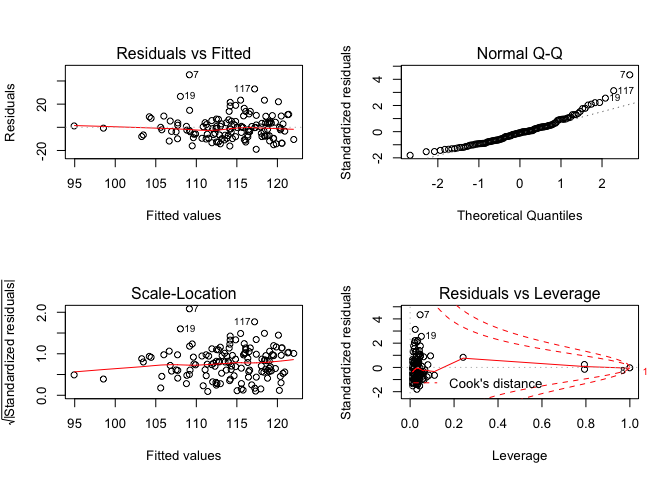
\includegraphics{descriptive_stats_files/figure-latex/unnamed-chunk-2-1.pdf}

Looking at outcomes distribution- sbp
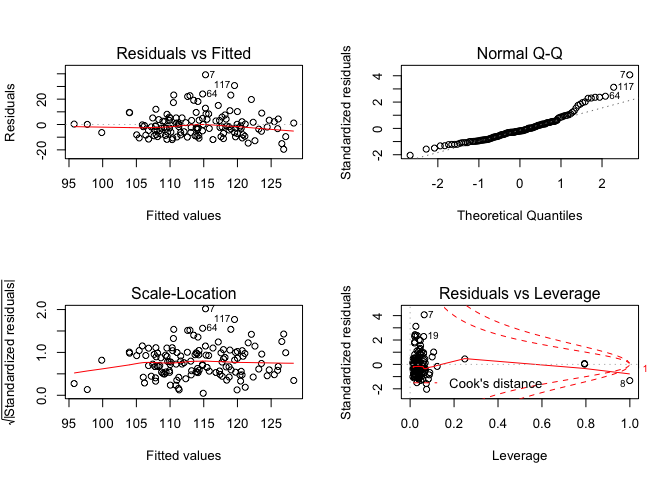
\includegraphics{descriptive_stats_files/figure-latex/unnamed-chunk-3-1.pdf}

Looking at outcomes distribution- dbp
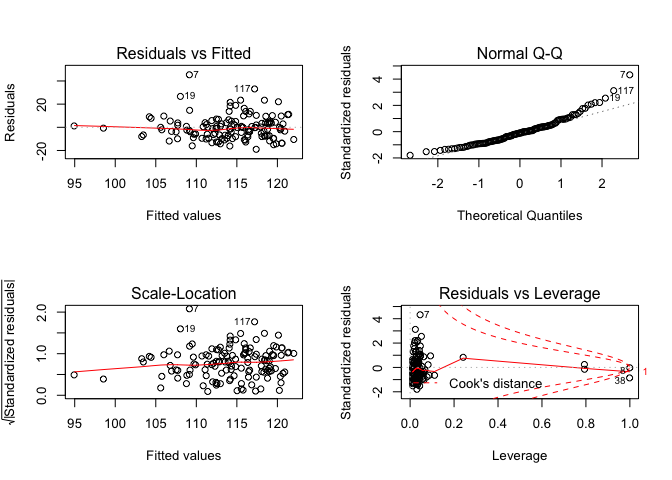
\includegraphics{descriptive_stats_files/figure-latex/unnamed-chunk-4-1.pdf}

Looking at outcomes distribution- bmi
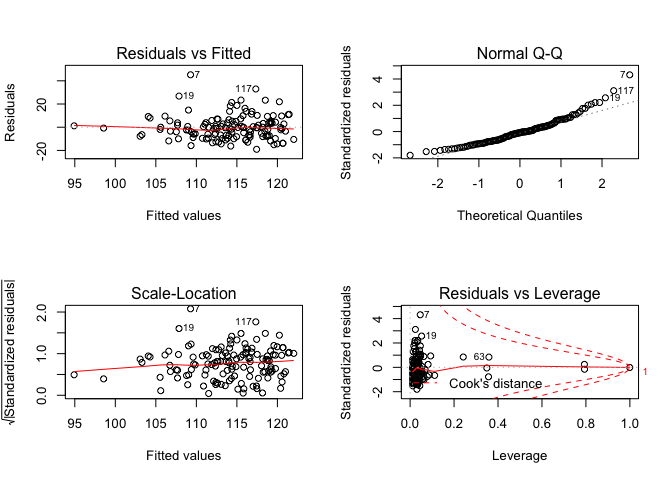
\includegraphics{descriptive_stats_files/figure-latex/unnamed-chunk-5-1.pdf}


\end{document}
